\documentclass{article}
\usepackage[utf8]{inputenc}

\title{Homework No.3}
\author{Osamu Katagiri-Tanaka : A01212611}
\date{\today}

% import math symbols
\usepackage{amsmath, esint}
\usepackage{cancel}

% import code snippets
\usepackage{listings}
\usepackage{xcolor}
\definecolor{codegreen}{rgb}{0,0.6,0}
\definecolor{codegray}{rgb}{0.5,0.5,0.5}
\definecolor{codepurple}{rgb}{0.58,0,0.82}
\definecolor{backcolour}{rgb}{0.99,0.99,0.96}
\lstdefinestyle{mystyle}{
    backgroundcolor=\color{backcolour},   
    commentstyle=\color{codegreen},
    keywordstyle=\color{magenta},
    numberstyle=\tiny\color{codegray},
    stringstyle=\color{codepurple},
    basicstyle=\ttfamily\small,
    breakatwhitespace=false,         
    breaklines=true,                 
    captionpos=b,                    
    keepspaces=true,                 
    numbers=left,                    
    numbersep=5pt,                  
    showspaces=false,                
    showstringspaces=false,
    showtabs=false,                  
    tabsize=2
}
\lstset{style=mystyle}

% import continuous lists
\usepackage{enumitem}

% format margins and paper size
\usepackage{geometry}
\geometry{
	paper         = a4paper, % Change to letterpaper for US letter
	inner         = 2.5cm,   % Inner margin
	outer         = 2.5cm,   % Outer margin
	bindingoffset = 0.5cm,   % Binding offset
	top           = 1.5cm,   % Top margin
	bottom        = 1.5cm    % Bottom margin
}

% import figure handler
\usepackage{graphicx}

% import references handler
\usepackage[
    style     = ieee,         % references format style
    backend   = biber,        % choose the processing program
    natbib    = true,         % enable additional reference formats
    citestyle = numeric-comp, % enable multiple citations
    sortcites = true,         % sort references in multiple citations
    sorting   = nyt           % sort the reference table
]{biblatex}
\addbibresource{references.bib}

% Note that ‘d’ in the differential is conventionally set in roman.
\newcommand{\ud}{\,\mathrm{d}}

% Paragraph spacing
\setlength{\parskip}{0.2cm}           % spacing between paragraphs
\renewcommand{\baselinestretch}{1.25} % spacing between lines

\begin{document}

\maketitle

\section{Problem Statement}

The equation of conservation of chemical species under a chemical reaction of
decomposition can be represented with the PDE given below.

$$ \frac{\partial C}{\partial t} = \vec{\nabla} \cdot (D \vec{\nabla} C) - \vec{v} \cdot \vec{\nabla} C - k C^n $$

If a tubular catalytic chemical reactor initially filled with an inert solvent $(C = 0)$ is fed by a stream of component ``A" with a concentration of $1 kmol/m^3$ $(C = 1)$ and speed of $1 m/s$ $(v = 1)$, calculate the distribution of ``A" across the reactor and as a function of time $C(x, t)$. The dispersion coefficient of the component ``A" is $0.02 m^2/s$ $(D = 0.01)$, the kinetic decomposition coefficient $0.05 s^{-1}$ $(k = 0.05)$. The chemical decomposition kinetics is first order $(n = 1)$.

\section{Sketch}

\begin{center}
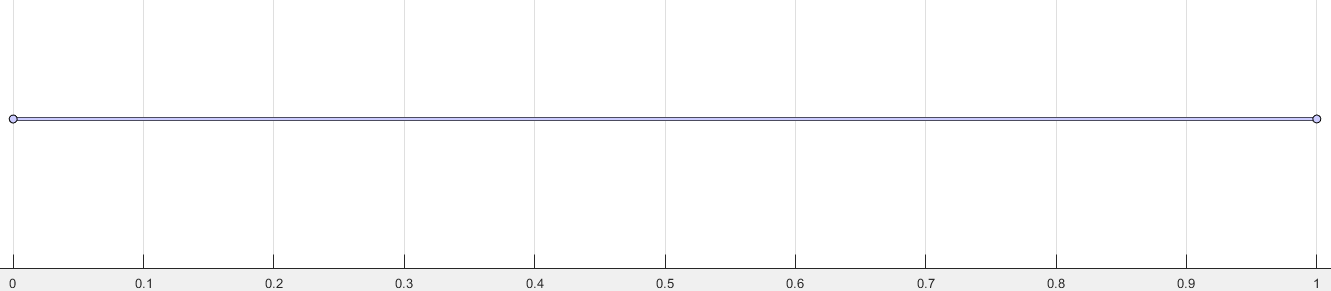
\includegraphics[width=\textwidth]{./img/Sketch.png}
\end{center}

\section{Assumptions and Approximations}

% You can assume 1-m long reactor

\section{Physical constants}

\section{Physical Transport or Thermodynamic Properties}

\section{Calculations}

The molar balance in axial direction for a 1D flow can be written as:

$$ \frac{\partial C}{\partial t} = D \frac{\partial^2 C}{\partial x^2} - v \frac{\partial C}{\partial x} - k C^n $$

The initial condition $IC$ is:
$$ \left. C \right|_{t = 0} = 0 \textrm{, } 0 \leq x \leq 1 $$

The boundary conditions $BCs$ are:
$$ \left. C \right|_{x = 0} = 1 \textrm{, } t > 0 $$
$$ \left. \frac{\partial C}{\partial t} \right|_{x = L} = 0 \textrm{, } t \geq 0 $$

Where, \\
$D$ is the diffusion coefficient \\
$C$ is the injection concentration \\
$v$ is the velocity of fluid injection \\
$k$ is the first order kinetic coefficient \\
$L$ is the length of domain \\
$t$ is the simulation time \\
$x$ is the distance mesh

\subsection{PDEPE solver}

The built in function PDEPE, solves a general problem of a 1-D (parabolic or elliptic) partial differential equation, for a Cartesian, cylindrical or spherical coordinates of the from:

$$ c \left( x, t, u, \frac{\partial u}{\partial x} \right) \frac{\partial u}{\partial t} = \frac{1}{x^m} \frac{\partial}{\partial x} \left( x^m f \left( x, t, u, \frac{\partial u}{\partial x} \right) \right) + s \left( x, t, u, \frac{\partial u}{\partial x} \right) $$

Where, \\
$\displaystyle m = 0$ represents the symmetry of the problem (0 for slab, 1 for cylindrical, or 2 for spherical) \\
$\displaystyle c = 1$ is a diagonal matrix \\
$\displaystyle f = D \frac{\partial u}{\partial x}$ is the flux term\\
$\displaystyle s = - v \frac{\partial u}{\partial x} - k u^n$ is the source term \\
$c$, $f$, and $s$ correspond to coefficients in the standard PDE equation form expected by pdepe. These coefficients are coded in terms of the input variables $x$, $t$, $u$, and $dudx$. Listing \ref{DiffusionPDEfun} implements a function that calculates the values of the coefficients $c$, $f$, and $s$.

\begin{lstlisting}[language=Matlab, caption=PDE function for equations, label=DiffusionPDEfun]
function [c, f, s] = DiffusionPDEfun(x, t, u, dudx, P)
    % Parameters
    D  = P(1);
    k  = P(3);
    vo = P(4);
    
    % PDE
    c = 1;
    f = D .* dudx;
    s = - k * u - vo * dudx;
end
\end{lstlisting}

PDEPE requires an `initial condition function', which is defined as a function that defines the initial condition. For $t = t_o = 0$ and all $x$, the solution satisfies the initial condition of the form:

$$ u(x, t_o) = u_o(x) $$

PDEPE calls the initial condition function with an argument $x$, which evaluates the initial values for the solution at $x$ in vector $u_o$. The number of elements in $u_o$ is equal to the number of equations. Listing \ref{DiffusionICfun} implements the constant initial condition.

\begin{lstlisting}[language=Matlab, caption=Initial condition function, label=DiffusionICfun]
function u0 = DiffusionICfun(x, P)
    % u0 = u0(x)
    u0 = 0;
end
\end{lstlisting}

The third function required by the PDEPE solver is the `boundary condition function'. The boundary condition function spefifies the boundary conditions for all $t$, the solution satisfy the boundary condition of the form:

$$ p(x, t, u) + q(x, t) f \left( x, t, u, \frac{\partial u}{\partial x} \right) = 0 $$

Listing \ref{DiffusionBCfun} implements a function that defines the terms $p$ and $q$ of the boundary conditions. $u1$ is the approximate solution of the left boundary, $ur$ is the approximate solution of the right boundary, $pl$ and $ql$ are vectors corresponding to $p$ and $q$ evaluated at $xl$, and $pr$ and $qr$ are vectors corresponding to $p$ and $q$ evaluated at $xr$.

\begin{lstlisting}[language=Matlab, caption=Boundary condition function, label=DiffusionBCfun]
function [pl, ql, pr, qr] = DiffusionBCfun(xl, u1, xr, ur, t, P)
    % BCs: No flux boundary at the right boundary and constant
    % concentration on the left boundary
    c0 = P(2);
    pl = u1 - c0;
    ql = 0;
    pr = 0;
    qr = 1;
end
\end{lstlisting}

Listing \ref{PDEPE_solver} calls the PDEPE solver with the parameters $P$ specified in the `Problem Statement' section. The PDE function of equations, initial condition function, and boundary condition function are passed to the \emph{pdepe()} function. Matlab's \emph{pdepe()} solves a system of PDEs with one spatial variable and time. The equations being solved are specified in Listing \ref{DiffusionPDEfun}, the initial value is coded in Listing \ref{DiffusionICfun}, and the boundary conditions are defined in Listing \ref{DiffusionBCfun}. The ODEs resulting from the discretization in space are integrated at the time values $t$. \emph{pdepe()} returns values of the solution on a mesh provided in $x$. 

\begin{lstlisting}[language=Matlab, caption=PDEPE solver, label=PDEPE_solver]
% Parameters
P(1) = 0.01;                    % Diffusion coefficient D
P(2) = 1.0;                     % Injection concentration c0
P(3) = 0.5;                     % First order kinetic coefficient k
P(4) = 1.0;                     % Velocity of fluid injection vo
L    = 1;                       % Length of domain
maxt = 1;                       % Max. simulation time
m    = 0;                       % Parameter corresponding to the symmetry
%                                 of the problem (0 for slab, 1 for
%                                 cylinder, or 2 for sphere)
step = 32;
t    = linspace(0, maxt, step); % Tspan
x    = linspace(0, L, step);    % xmesh

sol = pdepe(          ...
    m,                ...
    @DiffusionPDEfun, ... % Function containing the PDEs
    @DiffusionICfun,  ... % Function containing the ICs for t=0 at all x
    @DiffusionBCfun,  ... % Function containing the BCs for x=0 and x=L
    x,                ... % Spatial mesh
    t,                ... % Time span of integration
    [],               ... % Options
    P                 ... % Parameters
);

% ui(t,x) = (tspan(j),xmesh(k)).
u = sol;
\end{lstlisting}

Listings \ref{PDEPE_speciesDistancePlot} and \ref{PDEPE_speciesTimePlot} visualize \emph{pdepe()} return values. Figures \ref{fig_PDEPE_Species_vs_Distance} and \ref{PDEPE_Species_vs_Time} are the generated plots with the PDEPE results.

\begin{lstlisting}[language=Matlab, caption=PDEPE Distance vs. Species plot, label=PDEPE_speciesDistancePlot]
% plot limits
dlim = 0.02;
x_lim = [0 - dlim, L + dlim];
t_lim = [0 - dlim, maxt + dlim];
u_lim = [0 - dlim, P(2) + dlim];

figure
for n = linspace(1, step, step)
    hold all
    plot(x, u(n, :))
end
xlabel('Distance x')
ylabel('Species u')
axis([x_lim(1) x_lim(2) u_lim(1) u_lim(2)])
\end{lstlisting}

\begin{figure}[h!]
\centering
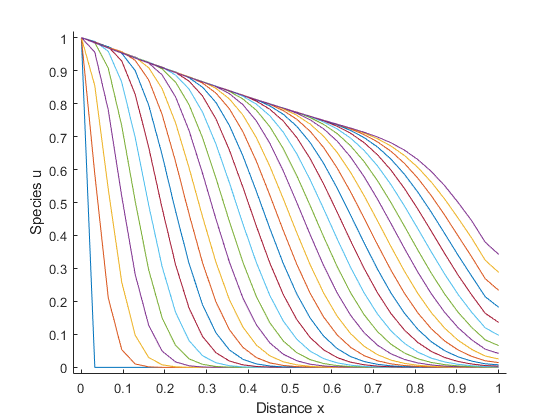
\includegraphics[width=0.75\textwidth]{./img/PDEPE_Species_vs_Distance.png}
\caption{PDEPE - Species vs. Distance}
\label{fig_PDEPE_Species_vs_Distance}
\end{figure}

\begin{lstlisting}[language=Matlab, caption=PDEPE Time vs. Species plot, label=PDEPE_speciesTimePlot]
figure
for n = linspace(1, step, step)
    hold all
    plot(t, u(:, n))
end
xlabel('Time t')
ylabel('Species u')
axis([t_lim(1) t_lim(2) u_lim(1) u_lim(2)])
\end{lstlisting}

\begin{figure}[h!]
\centering
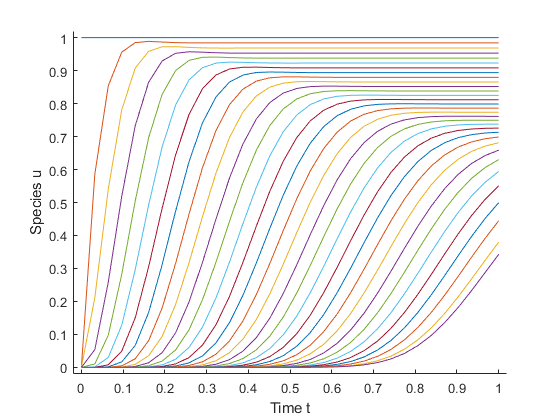
\includegraphics[width=0.75\textwidth]{./img/PDEPE_Species_vs_Time.png}
\caption{PDEPE - Species vs. Time}
\label{PDEPE_Species_vs_Time}
\end{figure}

\subsection{FEATool solver}

Problem statement can be also tacked using \emph{FEATool}. The following steps were taken to solve the ``tubular water treatment uv-light reactor

\textbf{Initialization and model selection:}
\begin{enumerate}
\item To start a new model click the New Model toolbar button, or select New Model... from the File menu.
\item Select the 1D radio button.
\item Select the Convection and Diffusion physics mode from the Select Physics drop-down menu.
\item Press OK to finish the physics mode selection.
\end{enumerate}

\begin{center}
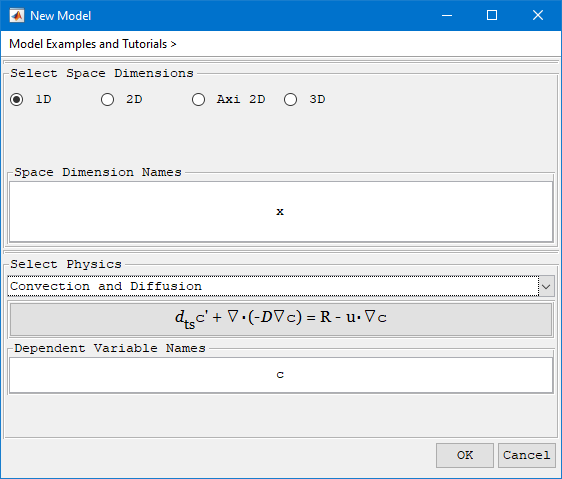
\includegraphics[scale=0.60]{./matlab/FEATool_steps/initializationAndModelSelection.png}
\end{center}

\textbf{Geometry definition:}
\begin{enumerate}[resume]
\item Press the Create line Toolbar button.
\item Press OK to finish and close the dialog box.
\end{enumerate}

\begin{center}
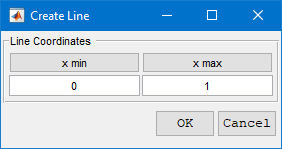
\includegraphics[scale=0.60]{./matlab/FEATool_steps/geometryDefinition.png}
\end{center}

\textbf{Grid specification:}
\begin{enumerate}[resume]
\item Switch to Grid mode by clicking on the corresponding Mode Toolbar button.
\item Enter  0.01  into the Grid Size edit field.
\end{enumerate}

\begin{center}
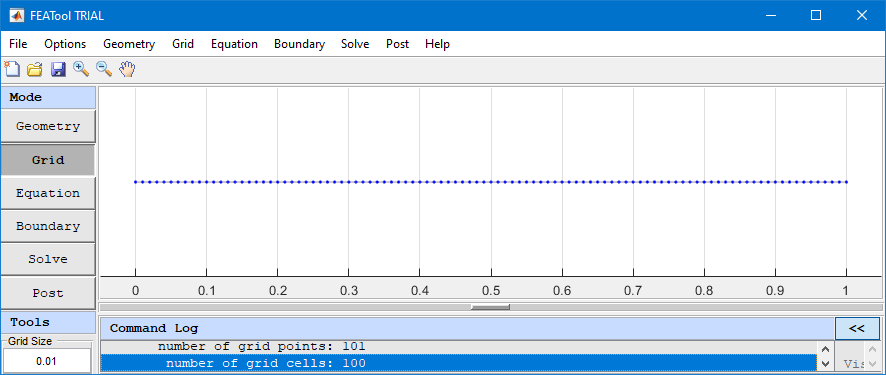
\includegraphics[scale=0.60]{./matlab/FEATool_steps/gridSpecification.png}
\end{center}

\textbf{PDE parameters and initial condition:}
\begin{enumerate}[resume]
\item Switch to Equation mode by clicking on the corresponding Mode Toolbar button.
\item Enter  0.1  into the Time scaling coefficient edit field.
\item Enter  0.01  into the Diffusion coefficient edit field.
\item Enter  1  into the Convection velocity in x-direction edit field.
\item Enter  0.0  into the Reaction rate edit field.
\item Press the Apply button.
\item Press OK to finish the equation and subdomain settings specification.
\end{enumerate}

\begin{center}
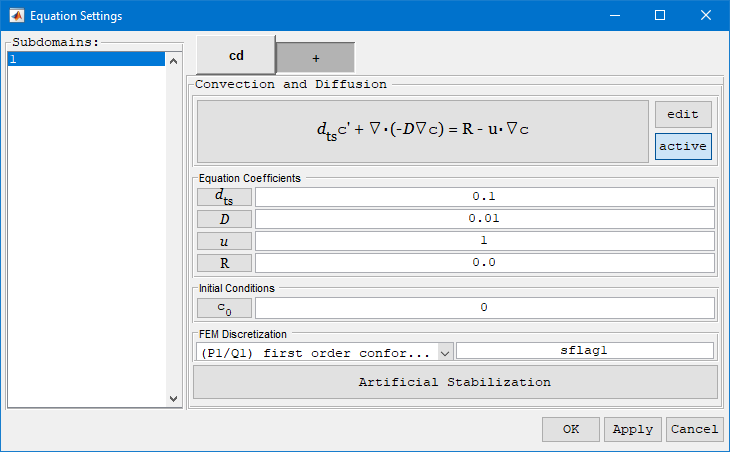
\includegraphics[scale=0.60]{./matlab/FEATool_steps/PDEparametersAndInitialCondition.png}
\end{center}

\textbf{Boundary conditions:}
\begin{enumerate}[resume]
\item Switch to Boundary mode by clicking on the corresponding Mode Toolbar button.
\item Select Concentration from the Convection and Diffusion drop-down menu.
\item Enter  1  into the Concentration edit field.
\item Select 2 in the Boundaries list box.
\item Press the Apply button.
\item Press OK to finish the boundary condition specification.
\end{enumerate}

\begin{center}
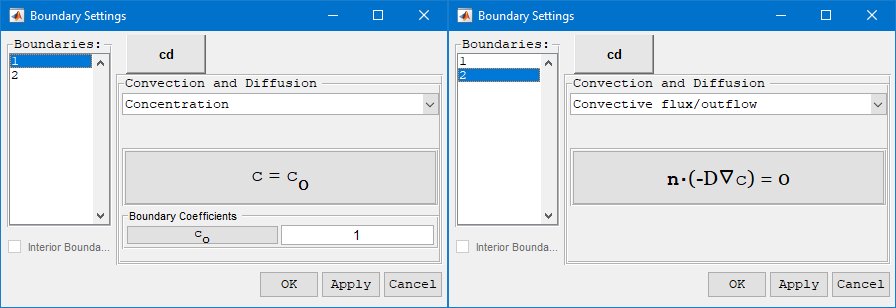
\includegraphics[scale=0.60]{./matlab/FEATool_steps/boundaryConditions.png}
\end{center}

\textbf{Solver settings:}
\begin{enumerate}[resume]
\item Switch to Solve mode by clicking on the corresponding Mode Toolbar button.
\item Press the Settings Toolbar button.
\item Select Time-Dependent from the Solution and solver type drop-down menu.
\item Enter  30  into the Maximum number of non-linear iterations edit field.
\item Enter  0.001  into the Time step size edit field.
\item Enter  0.001  into the Duration of time-dependent simulation (maximum time) edit field.
\item Press the Solve button.
\end{enumerate}

\begin{center}
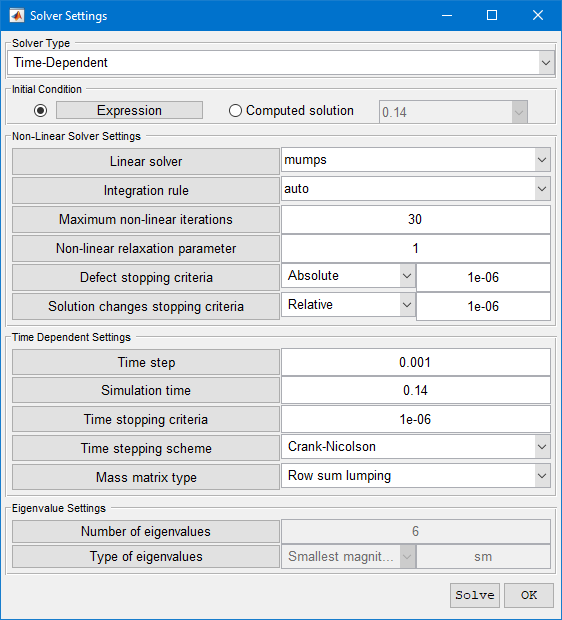
\includegraphics[scale=0.60]{./matlab/FEATool_steps/solverSettings.png}
\end{center}

\textbf{Solve for different time values:}
\begin{enumerate}[resume]
\item \label{itm_first} Switch to Solve mode by clicking on the corresponding Mode Toolbar button.
\item Press the Settings Toolbar button.
\item Enter  0.010  into the Duration of time-dependent simulation (maximum time) edit field.
\item \label{itm_last} Press the Solve button.
\item[] Repeat steps \ref{itm_first} through \ref{itm_last} for different values of "Duration of time-dependent simulation (maximum time)" from 0.020 to 0.140 with 0.010 increments
\end{enumerate}

\begin{figure}[h!]
\centering
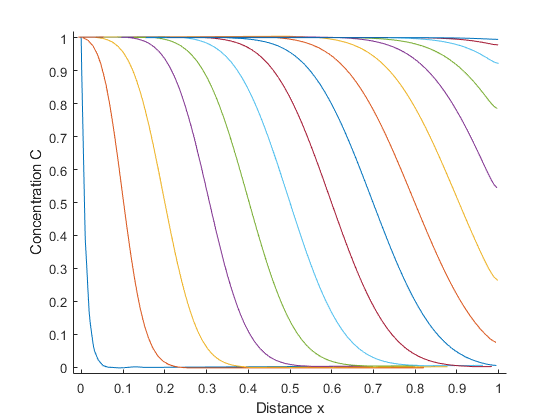
\includegraphics[width=0.75\textwidth]{./img/FEATool_Concentration_vs_Distance.png}
\caption{FEATool - Concentration vs. Distance for time t = [0.001, 0.140]}
\label{fig_PDEPE_Species_vs_Distance}
\end{figure}

\section{Discussion}

\printbibliography[title={References}]
\end{document}